\documentclass[pdf]
{beamer}
\mode<presentation>{}
%% preamble
\title{Model inference from protein time-course in Hematopoietic Stem Cells (HSC)}
\subtitle{}
\author[shortname]{Pandu Raharja \inst{1, 2} \and Rene Schoeffel \inst{1, 2} \and Michael Strasser \inst{3}}
\institute[shortinst]{\inst{1} Technische Universit\"at M\"unchen \and %
                      \inst{2} Ludwig-Maximilians-Universit\"at M\"unchen \and %
                      \inst{2} Institute of Computational Biology (ICB), Helmholtz Zentrum M\"unchen}
\begin{document}

%% title frame
\begin{frame}
\titlepage
\end{frame}

%% normal frame
\begin{frame}{Introduction}
	\begin{itemize}
		\item Dynamics of hematopoetic stem cell maturation cell from Common Myeloid Progenitor (CMP) to Megakaryocyte-Erythroid Progenitor (MEP) and Granulocyte-Macrophage Progenitor (GMP)
	\end{itemize}
	
	\begin{figure}[ht]
		\begin{center}
			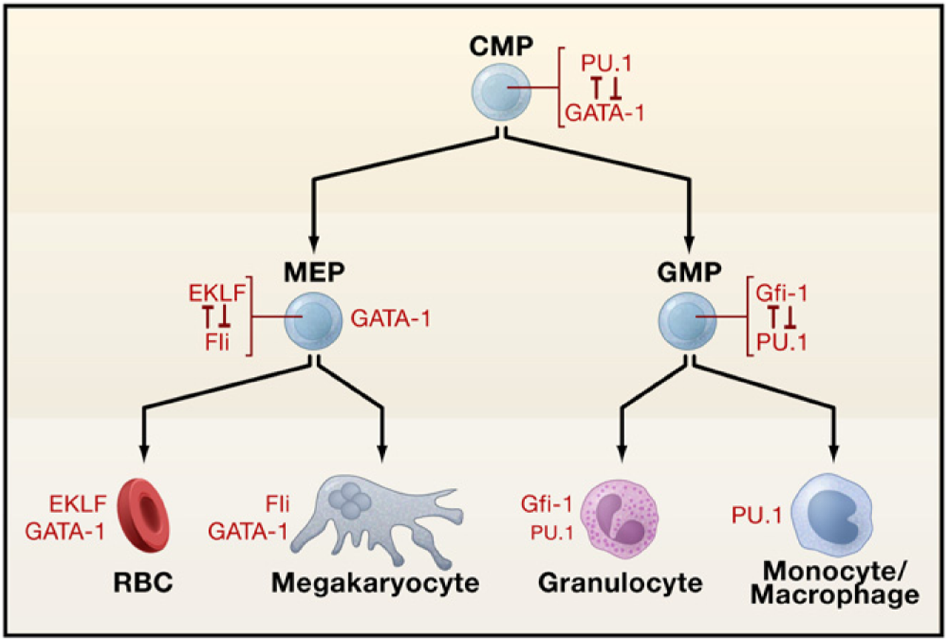
\includegraphics[height=2in]{figures/homatopoietic_focus.png}
			~\footnote{Graf \& Enver, 2009, \textit{Nature}}
		\end{center}
	\end{figure}
\end{frame}

\begin{frame}{Introduction (cont'd)}
	\begin{itemize}
	\item MEP and GMP yield not 50\% : 50\% as previously thought, but 70\% : 30\%
	\item Assumed dynamics between \texttt{Pu.1} and \texttt{Gata1} in cell maturation fate
	\begin{itemize}
		\item Dynamics assumed to be a bistable toggle-switch system
	\end{itemize}
	\item Analysis on single-cell time-lapsed data
	\end{itemize}
	\begin{figure}[ht]
		\begin{center}
			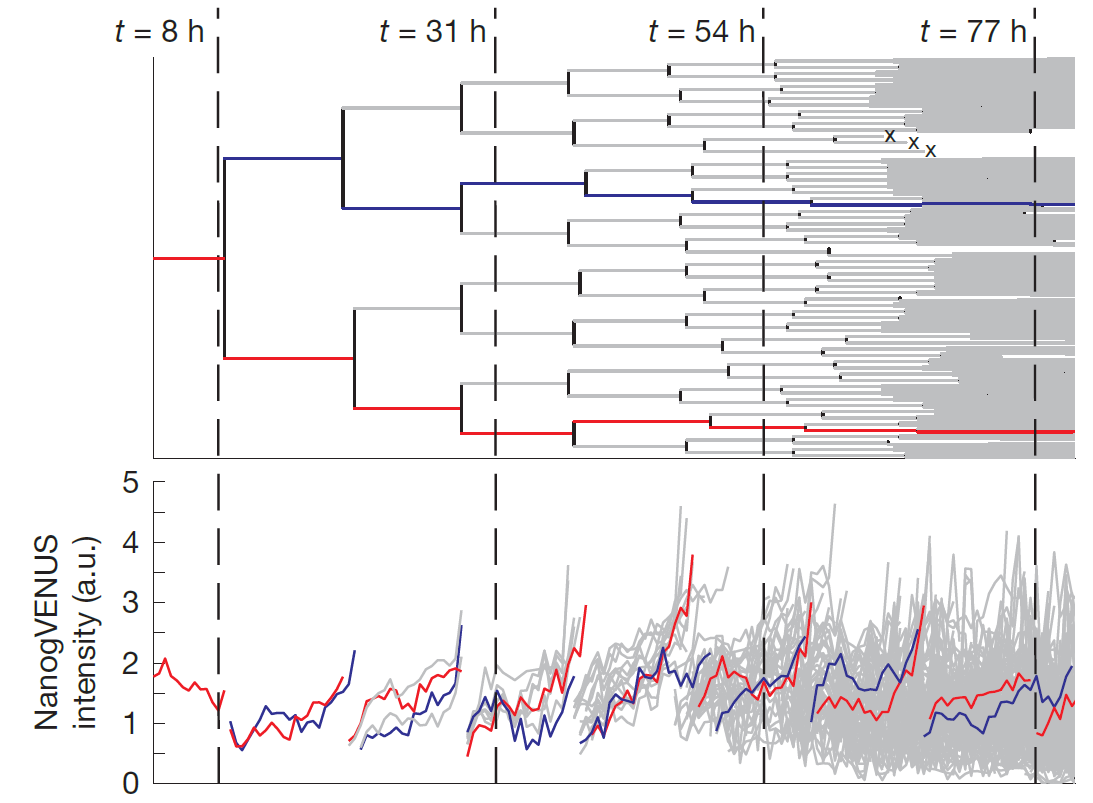
\includegraphics[height=1.5in]{figures/cell-generations.png}
			~\footnote{Feigelman, 2016, Ph.D. Thesis}
		\end{center}
	\end{figure}
\end{frame}

\begin{frame}{Problems}
	\begin{itemize}
	\item Stochaticity in single cell resolution is more punctuated
	\item Tree structure of the data add ore complexity: inheritance of information during inference process is not trivial
	\end{itemize}
\end{frame}

\begin{frame}{Ideas}
	\begin{itemize}
	\item Sequential Monte Carlo simulations along the time-apsed data to infer "good" parameters
	\item<2-> \textbf{problem:} Overfitting due to single-cell biased
	\item<3-> \textbf{solution:} Inference across cell lineages
	\item<4-> Inferred parameters from all simulated lineages are represented as distribution
	\item<5-> Final inferred parameters are expected value $E$ of the distribution
	\end{itemize}
\end{frame}

\begin{frame}{Particle Filtering (6)}

\end{frame}

\begin{frame}{Particle Filtering (7)}

\end{frame}

\begin{frame}{Particle Filtering: algorithm}
	\begin{enumerate}
		\item Initialization of parameters $\theta$.
		\item Input of data $\mathcal{D}$.
		\item Particle filtering routine:

		\begin{enumerate}
			\item Generation of initial particles for step i
			
			\begin{equation}
				Ki := (K_{i1}, K_{i2}, \dots, K_{im})
			\end{equation}

			\item Simulation run of each particle $K_{ij}$
			\item Weighting of each particle. The weight is a function of the probability of observing the data given the simulation result.

			\begin{equation}
				w_i^k = P(D_i | X_i^k) = \mathcal{N}(\mathcal{D}_i | X_i^k)
			\end{equation}

			\item Parameter update for every K,

			\begin{equation}
				\theta^k \propto P(\theta | X^k_{[to, ti]})\label{eq:13}
			\end{equation}

		\end{enumerate}

		\item Model comparison.

	\end{enumerate}
\end{frame}

\begin{frame}{Particle Filtering: visualization}
	\begin{figure}[ht]
		\begin{center}
			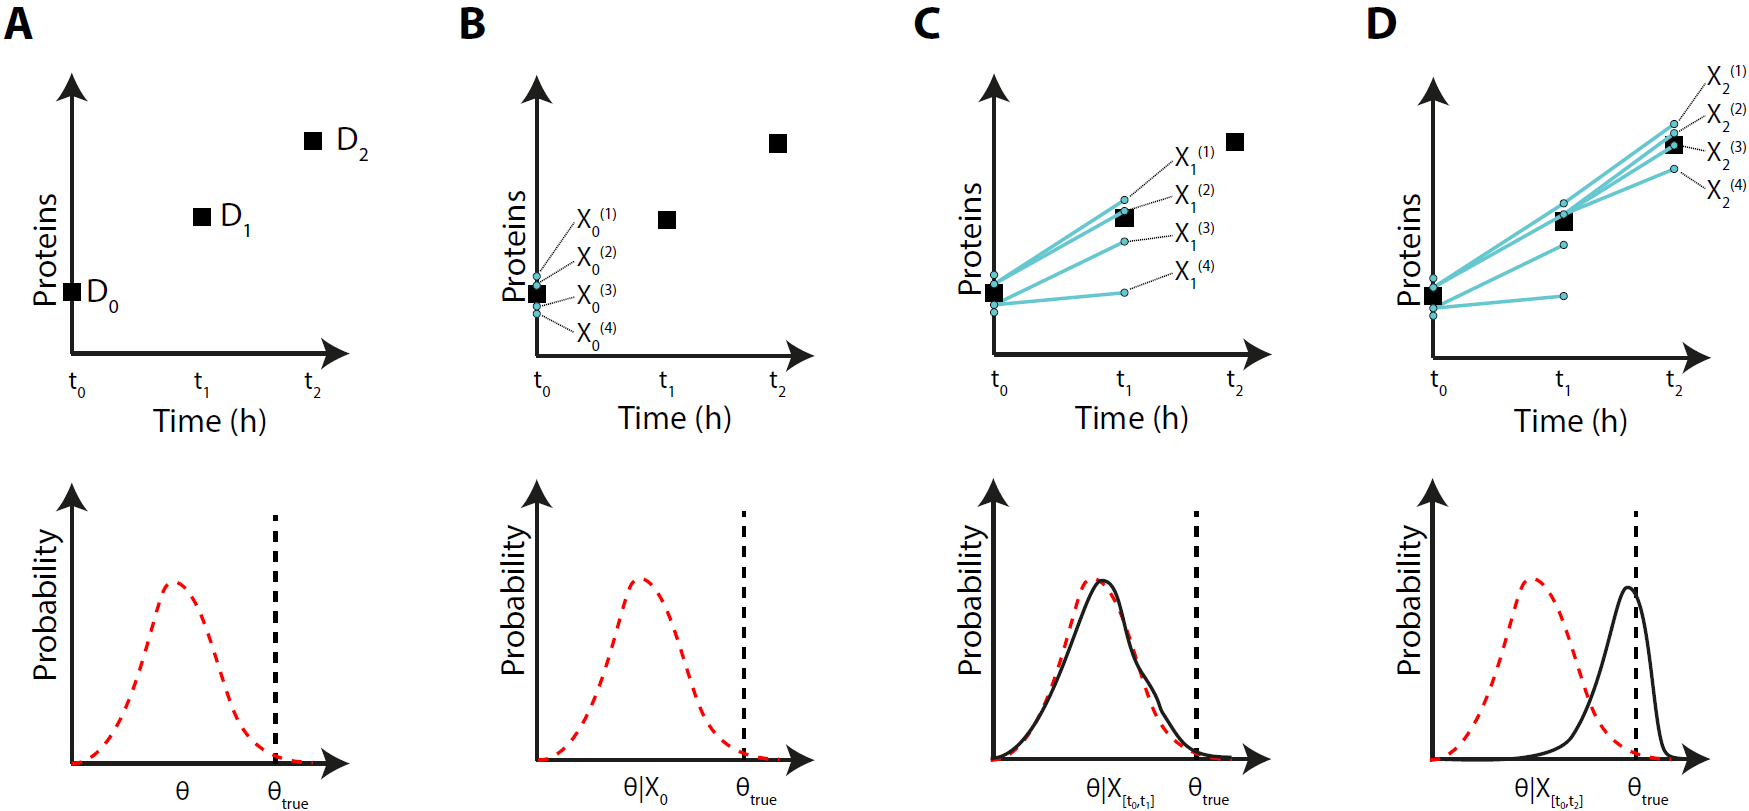
\includegraphics[height=2in]{figures/particle_filtering.png}
			~\footnote{Feigelman, 2016, Ph.D. Thesis}
		\end{center}
	\end{figure}
\end{frame}

\end{document}